\chapter{Visualization System}
In this chapter the system architecture and corresponding components will be introduced. This chapter emphasizes on depicting the whole picture of the solution, some specific technical detail will be represented in the later chapters.   

\section{System architecture}

The main role of visualization system is to handle and process the data between different components and represent them in graphics. The flowchart in fig. 1 shows the visualization pipeline in a general visualization system\citeRefs{dosSantos2004311}.

\begin{figure}[htb]
  \centering
  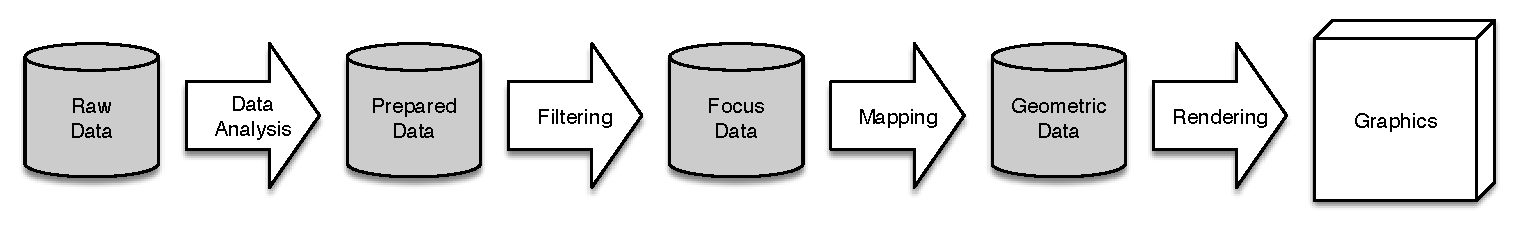
\includegraphics[width=.9\textwidth]{Assets/Visualization_Pipeline}
  \caption{Visualization pipeline}
\end{figure}

The data flow is abstracted out in several state 

\section{Work flow between system components}